\documentclass[11pt,a4paper]{article}
\usepackage[T1]{fontenc}
\usepackage[utf8]{inputenc}
\usepackage{lmodern}
\usepackage[a4paper,margin=25mm,headheight=15pt]{geometry}
\usepackage{amsmath,amssymb,amsthm,mathtools}
\usepackage{microtype,graphicx,booktabs,longtable,array,tabularx}
\usepackage{enumitem,xcolor,xurl,fancyhdr}
\definecolor{ink}{HTML}{18374C}
\definecolor{accent}{HTML}{087F8C}
\usepackage[colorlinks=true,linkcolor=ink,citecolor=accent,urlcolor=accent,
 pdftitle={Summation and Singularities under Polylogarithmic Reversion},
 pdfauthor={Research manuscript prepared for the ProveIt project}]{hyperref}
\newtheorem{theorem}{Theorem}[section]
\newtheorem{proposition}[theorem]{Proposition}
\newtheorem{lemma}[theorem]{Lemma}
\newtheorem{corollary}[theorem]{Corollary}
\theoremstyle{definition}
\newtheorem{definition}[theorem]{Definition}
\newtheorem{example}[theorem]{Example}
\theoremstyle{remark}
\newtheorem{remark}[theorem]{Remark}
\numberwithin{equation}{section}
\setlist{itemsep=3pt,topsep=5pt}
\setlength{\emergencystretch}{2em}
\setlength{\parskip}{3pt}
\newcommand{\C}{\mathbb C}
\newcommand{\R}{\mathbb R}
\newcommand{\N}{\mathbb N}
\newcommand{\Q}{\mathbb Q}
\DeclareMathOperator{\Li}{Li}
\DeclareMathOperator{\ord}{ord}
\newcommand{\repo}{\textsf{ProveIt}}
\newcolumntype{P}[1]{>{\raggedright\arraybackslash}p{#1}}
\pagestyle{fancy}
\fancyhf{}
\fancyhead[L]{\small\itshape Polylogarithmic reversion}
\fancyhead[R]{\small Summation and singularities}
\fancyfoot[C]{\thepage}
\renewcommand{\headrulewidth}{0.3pt}
\title{\color{ink}\bfseries Summation and Singularities under\\
Polylogarithmic Reversion\\[6pt]
\large\mdseries Convergent angular reconstruction, sharp Lambert late terms,\\
and removable inverse endpoints}
\author{Research manuscript prepared for the \repo\ project}
\date{12 October 2026\\[3pt]\small Repository baseline:
\texttt{8f5afd4d7565df808359f6a0c22f87f79a119bb9}}
\begin{document}
\maketitle
\begin{abstract}
We investigate three ways in which inversion changes a polylogarithmic
expansion. First, the harmonic depth-two angular-zero transseries is known
to diverge even after equal exponential bases are collected. We construct
a specified summation of its original multiset coefficient family:
sum each nonlinear degree at subunit radius, take its radial Abel limit,
and then sum the degree blocks. For every real $a\ge6$, $b>0$, and
$0<\rho\le1$, this last series converges absolutely to the actual angular
displacement, with a uniform explicit geometric error bound. At integer orders
all its coefficients belong to one fixed finitely generated algebra of
polylogarithm values. A finite frequency-and-degree truncation attains
$\exp(-\lambda a^2+O_\lambda(a))$ error for every
$0<\lambda<\log(3/2)$.

Second, we prove the precise even/odd late-coefficient conjecture in the
new resonant Lambert inverse report. Uniform factorial convolution
estimates control the previously unjustified summation over the number
of factors. We obtain a first correction, a universal leading-amplitude
law for analytic inverse cores, and an exact initial-disk Borel
decomposition into two logarithms and two dilogarithms with a continuously
differentiable remainder. Both nearest Borel endpoints are singular for
every nonzero complex coupling.

Third, we classify the minimal endpoint ramification of the direct
inverse of $\Li_s$ for every real $s>1$. Its endpoint is holomorphic
exactly at $s=1+1/q$, $q\ge2$ integral. We give its convergent Taylor
charts and disprove a proposed all-real-order extension of an
integer-order cut-modulus inequality. Classical ingredients and previous
repository results are attributed; proofs, finite exact checks, and
ordinary numerical diagnostics retain distinct scopes.
\end{abstract}
\noindent\textbf{Keywords.} Polylogarithm; harmonic sums; transseries;
Lagrange inversion; Abel summation; factorial asymptotics; Borel transform;
ramification; Lambert series.
\newpage
\begingroup\setlength{\parskip}{0pt}\tableofcontents\endgroup
\newpage

\section{Questions, conclusions, and provenance}
\label{sec:scope}

An inverse expansion has several distinct mathematical meanings. A
formal coefficient formula can be valid without its sum converging.
A convergent analytic representation can require a different grouping
from the original asymptotic scale. The nearest singularities of a
Borel transform depend on exact late coefficients, while a branch point
of the forward function can disappear from its inverse. This article
addresses these distinctions in concrete problems drawn from the
intersection of \repo's Polylogarithms and Transseries projects.

The source baseline is the commit displayed on the title page, inspected
on 12 October 2026. In particular, the three then-current incoming
archives were read before selecting the research targets. The article
does not treat earlier unanswered questions as unanswered without
checking those arrivals. The accompanying provenance file records exact
repository paths and archive members, so that the contribution remains
reviewable after the reports are moved into their canonical locations.

\subsection{The three research targets}

The angular-zero report~\cite{RepoAngular} supplies an explicit
multiset-indexed expansion with an error after every fixed finite
exponential cutoff. Its continuation~\cite{RepoFormal} proves that the
complete expansion diverges at every fixed integer outer order, even
after equal rational bases are combined. Research question 14 of that
continuation asks for a justified summation method. We answer it for
all real $a\ge6$ by an Abel limit within each fixed nonlinear degree,
followed by an ordinary convergent sum over degrees
(Theorem~\ref{ang:thm:sum}). The estimate comes from an actual
holomorphic norm on a fixed complex disk, not from differentiation of
a boundary Fourier series beyond its convergence range.

Question 13 of the same continuation asks for optimal moving
truncation. We give a rigorously controlled finite approximation with
an error that is Gaussian in the large outer order
(Theorem~\ref{ang:thm:gaussian}). This is a constructive upper bound
for a specified double cutoff. We do not identify the sharp optimum
for truncation in the original exponential-base ordering.

The incoming resonant Lambert inverse report~\cite{RepoLambert}
proves the exact inverse coefficient formula and its sharp Borel
radius for positive real coupling. Equations
\texttt{eq:conj-even} and \texttt{eq:conj-odd} there explicitly
conjecture the leading hyperbolic amplitudes. Section~\ref{lm:sec:main}
proves them with a locally uniform complex-parameter remainder and
one further term. The estimates are uniform in the number of
Lagrange factors, closing the exact gap identified by that report.

Finally, the convergent noninteger charts in
\cite[\texttt{prop:noninteger}]{RepoInverse} permit a sharper local
question: what is the \emph{smallest} branched cover required by the
inverse at $w=\zeta(s)$? Theorem~\ref{ep:thm:classification} answers
it for every real $s>1$. The exceptional holomorphic family also
clarifies why the real-order endpoint geometry cannot be inferred
from the integer-order theorem.

\subsection{Relation to established theory}

Lagrange inversion, including the auxiliary-parameter version used
here, is classical; Gessel's survey~\cite{Gessel} gives its formal
versions and proofs. Our use of Rouch\'e's theorem supplies the
additional analytic domain and quantitative bounds needed for the
angular summation. The positive depth-two kernel and global
angular-zero uniqueness are already repository results
\cite{RepoThreshold}; we rederive the kernel moments because their
uniform estimates are central to the new argument.

The general theory of factorially divergent series is also established.
Borinsky~\cite{Borinsky}, building on earlier work including Bender,
develops product, composition, and inverse rules for such series.
Our elementary convolution proof is consistent with that framework.
Its role is to prove the specific two-action Lambert conjecture, retain
uniformity in the complex coupling, and make the first correction and
initial-disk Borel regularity explicit. Neither factorial reversion
itself nor the general existence of resurgent Lambert expansions is
claimed as new. For the latter, see Dorigoni--Kleinschmidt~\cite{DK}.

The direct inverse classification uses the classical convergent
Jonqui\`ere expansion~\cite{DLMF}. It sharpens the repository's
existing two-variable charts; the general mechanism of Puiseux
uniformization is classical. The newest quadratic-feedback
arrival~\cite{RepoQuadratic} contains related minimal-ramification
calculations for a different implicit function. We credit this
nearby precedent and distinguish the direct inverse studied here.

Accordingly, the novelty claim is specific: these are proved answers
and refinements relative to the inspected corpus, supported by a
targeted primary-source search. No exhaustive worldwide priority
claim is made for every corollary or special-case identity.

\subsection{Conventions and evidence}

All logarithms are continued from their explicitly specified real
branches. The shifted Borel transform is
\[
 \mathcal B\left(\sum_{n\ge1}c_nq^n\right)(\xi)
   =\sum_{n\ge1}\frac{c_n}{\Gamma(n)}\xi^{n-1}.
\]
An estimate locally uniform in $u$ means uniform on every compact
subset of the stated parameter domain. Statements about a holomorphic
function inside a disk and continuous boundary values do not imply
analytic continuation across the boundary.

Every theorem below has a conventional proof. The supplied programs
check finite algebraic identities and evaluate independent numerical
diagnostics. The decimals are not interval enclosures, and the
programs are not proof-assistant formalizations. This manuscript was
prepared with AI assistance; it is intended for mathematical review
before incorporation into a collective manuscript.

\section{A complex neighborhood for the harmonic angular equation}
\label{ang:sec:kernel}

For real $a,b>0$ define, initially in the unit disk,
\begin{equation}
 F_{a,b}(z)=\sum_{n\ge2}\frac{H_{n-1}^{(b)}}{n^a}z^n,
 \qquad H_m^{(b)}=\sum_{j=1}^m j^{-b}.
 \label{ang:eq:F}
\end{equation}
This is the depth-two polylogarithm $\Li_{a,b}(z,1)$ when the
multiple-polylogarithm convention uses $n>m\ge1$ and the factor $z^n$.
The elementary inequality $1\le H_m^{(b)}\le m$ will be used
uniformly over all $b>0$.

\begin{lemma}[Positive kernel and exact moments]
\label{ang:lem:kernel}
On $\C\setminus[1,\infty)$,
\begin{equation}
 F_{a,b}(z)=z^2\int_{0<y<x<1}
 \frac{W_{a,b}(x,y)}{(1-xz)(1-yz)}\,dy\,dx,
 \quad
 W_{a,b}(x,y)=
 \frac{(-\log x)^{a-1}(\log(x/y))^{b-1}}{\Gamma(a)\Gamma(b)}.
 \label{ang:eq:kernel}
\end{equation}
For nonnegative integers $j,k$ its moments are
\begin{equation}
 \int_{0<y<x<1}W_{a,b}(x,y)x^jy^k\,dy\,dx
   =\frac1{(j+k+2)^a(k+1)^b}.
 \label{ang:eq:moments}
\end{equation}
\end{lemma}
\begin{proof}
Set $x=e^{-t}$ and $y=e^{-t-v}$. The Jacobian is $xy$, and the
integral in \eqref{ang:eq:moments} separates into Gamma integrals
with decay rates $j+k+2$ and $k+1$. Expanding both geometric
denominators in \eqref{ang:eq:kernel}, the coefficient of $z^n$
is
\[
 \sum_{k=0}^{n-2}\frac1{n^a(k+1)^b}
 =\frac{H_{n-1}^{(b)}}{n^a}.
\]
Absolute convergence justifies this computation for $|z|<1$.
On every compact subset of the slit plane the denominators are bounded
away from zero, and $W$ has finite mass $2^{-a}$. Dominated
convergence and differentiation on compact sets give the holomorphic
continuation. This is the kernel of \cite{RepoThreshold}, with its
moments made explicit for later estimates.
\end{proof}

For $a\ge6$, $b>0$, and $0<\rho\le1$, let $\theta_{a,b}(\rho)$ be the unique zero
in $(0,\pi)$ of $\operatorname{Im}F_{a,b}(\rho e^{i\theta})$.
In the range needed here its existence and simplicity follow from
the global angular theorem of \cite{RepoThreshold}; alternatively,
the construction below independently gives the root near $\pi/2$.
Write
\[
 \delta_{a,b}(\rho)=\frac\pi2-\theta_{a,b}(\rho).
\]
The Gaussian sign in the same source puts this displacement in
$(0,\pi/2)$. We shall also see its local positivity directly.

Set
\begin{align}
 R_{a,b}(z)&=F_{a,b}(z)-2^{-a}z^2,\notag\\
 z_+(v)&=i\rho e^{-iv},\qquad z_-(v)=-i\rho e^{iv},\notag\\
 S(v)&=\frac{2^a}{2i\rho^2}
       \bigl(R_{a,b}(z_+(v))-R_{a,b}(z_-(v))\bigr),
 \label{ang:eq:S}\\
 B(v)&=\frac{v}{\sin2v},\qquad B(0)=\frac12,
 \qquad f(v)=-B(v)S(v).
 \label{ang:eq:f}
\end{align}
These definitions are holomorphic; the difference in \eqref{ang:eq:S}
is used instead of taking an imaginary part at complex $v$.
For real $v$ it equals the normalized imaginary tail. The angular
equation is exactly
\begin{equation}
 \sin2v+S(v)=0.
 \label{ang:eq:angular}
\end{equation}

\begin{lemma}[Uniform analytic tail bound]
\label{ang:lem:norm}
Let $0<r<\pi/2$ and $c=\cos r$. On the disk $|v|\le r$,
\begin{equation}
 |S(v)|\le
 \rho e^{3r}\bigl(c^{-2}+2^{-b}c^{-1}\bigr)(2/3)^a.
 \label{ang:eq:norm}
\end{equation}
At $r=1/4$ this implies
\begin{equation}
 \sup_{|v|\le1/4}|f(v)|<\frac14\eta_{a,\rho},
 \qquad \eta_{a,\rho}=10\rho(2/3)^a.
 \label{ang:eq:eta}
\end{equation}
In particular $a\ge6$ gives $\eta_{a,\rho}\le640/729<1$.
\end{lemma}
\begin{proof}
If $z$ lies in either sector of half-width $r$ about $i$ or $-i$,
then $|1-tz|\ge\cos r=c$ for every $t\ge0$: this is the
distance from $1$ to a ray whose angle is at least $\pi/2-r$ in
absolute value. The elementary identity
\[
 \frac1{(1-A)(1-C)}-1
 =\frac{A}{(1-A)(1-C)}+\frac{C}{1-C}
\]
and the moments of $Wx$ and $Wy$ give
\[
 |R_{a,b}(z)|
 \le |z|^3 3^{-a}\bigl(c^{-2}+2^{-b}c^{-1}\bigr).
\]
For $|v|\le r$, both $z_\pm(v)$ lie in these sectors and have
modulus at most $\rho e^r$. Substitution proves
\eqref{ang:eq:norm}.

For completeness the constants can be bounded rationally:
\[
 \cos(1/4)>31/32,\qquad e^{3/4}<17/8,
 \qquad \sup_{|v|\le1/4}|B(v)|<8/15.
\]
The last inequality follows from
$|\sin(2v)/(2v)-1|\le\sinh(1/2)/(1/2)-1<1/16$.
For that strict bound the positive tail is at most
$(1/24)/(1-1/80)=10/237<1/16$.
Taylor's formula and a geometric bound on its positive tail give
$e^{3/4}<18427/8704<17/8$; the cosine bound follows from
$\cos x>1-x^2/2$. Consequently
\[
 4\sup|B|e^{3/4}(c^{-2}+c^{-1})
 <\frac{45696}{4805}<10.
\]
This proves \eqref{ang:eq:eta}, including its strictness.
\end{proof}

\section{A convergent summation of the angular multiset transseries}
\label{ang:sec:summation}

The scalar parameter used below scales the complete perturbation
before taking boundary values. It is not an independent variation of
infinitely many Fourier coefficients. Define the coupled equation
\begin{equation}
 \delta(\tau)=\tau f(\delta(\tau)),\qquad \delta(0)=0.
 \label{ang:eq:coupling}
\end{equation}

\begin{theorem}[Convergent angular reconstruction]
\label{ang:thm:sum}
For real $a\ge6$, $b>0$, and $0<\rho\le1$, put
\begin{equation}
 D_k(a,b;\rho)=\frac1k[v^{k-1}]f(v)^k
 =\frac{(-1)^k}{k}[v^{k-1}]B(v)^kS(v)^k.
 \label{ang:eq:D}
\end{equation}
Then
\begin{equation}
 \delta_{a,b}(\rho)=\sum_{k\ge1}D_k(a,b;\rho)
 \label{ang:eq:sum}
\end{equation}
converges absolutely. More precisely,
\begin{align}
 |D_k(a,b;\rho)|&\le\frac{\eta_{a,\rho}^k}{4k},
 \label{ang:eq:D-bound}\\
 \left|\delta_{a,b}(\rho)-\sum_{k=1}^KD_k(a,b;\rho)\right|
 &\le\frac{\eta_{a,\rho}^{K+1}}
 {4(K+1)(1-\eta_{a,\rho})},\qquad K\ge0.
 \label{ang:eq:sum-error}
\end{align}
The solution of \eqref{ang:eq:coupling} is holomorphic on
$|\tau|<\eta_{a,\rho}^{-1}$, which contains $\tau=1$.
\end{theorem}
\begin{proof}
On $|v|=1/4$, Lemma~\ref{ang:lem:norm} gives
$|\tau f(v)|<|v|$ when $|\tau|\eta_{a,\rho}<1$.
Rouch\'e's theorem shows that $v-\tau f(v)$ has exactly one
zero, counted with multiplicity, in the disk. It is therefore simple.
The implicit function theorem and uniqueness patch its local branches
into one holomorphic function of $\tau$ on the indicated disk.
Lagrange inversion gives \eqref{ang:eq:D}.
Applying Cauchy's coefficient estimate to $f(v)^k$ on the fixed
circle gives
\[
 |D_k|\le\frac1k(1/4)^{1-k}
              (\eta_{a,\rho}/4)^k
 =\frac{\eta_{a,\rho}^k}{4k}.
\]

At real $\tau$ the zero is real by conjugation symmetry. Moreover,
$S(0)<0$. Indeed the imaginary part of the positive kernel at
$z=i\rho$ is strictly negative: $z^2=-\rho^2$, while
the imaginary part of $((1-i\rho x)(1-i\rho y))^{-1}$ is
strictly positive for $0<y<x<1$. The removed quadratic term is
real. Thus $f(0)>0$, the zero starts positive for small positive
$\tau$, and it cannot cross zero for any $\tau>0$.
At $\tau=1$ it is in $(0,1/4)$ and solves the actual angular
equation. Global angular uniqueness identifies it with the stated
$\delta_{a,b}(\rho)$. Finally summing
$\sum_{k>K}\eta^k/k\le\eta^{K+1}/((K+1)(1-\eta))$
proves the error bound.
\end{proof}

\subsection{The exact summation order}

A multiset of Fourier modes is a finitely supported sequence
$\boldsymbol m=(m_3,m_4,\ldots)$ of nonnegative integers. Set
\[
 k=|\boldsymbol m|=\sum m_n,\quad
 \Lambda(\boldsymbol m)=\prod_{n\ge3}(n/2)^{m_n},\quad
 R(\boldsymbol m)=\sum_{n\ge3}(n-2)m_n,
 \quad h_n=H_{n-1}^{(b)}.
\]
The source coefficient is
\begin{equation}
 C(\boldsymbol m)=\frac{(-1)^k(k-1)!}{\prod m_n!}
 [v^{k-1}]B(v)^k
 \prod_{n\ge3}\sin(n\pi/2-nv)^{m_n}.
 \label{ang:eq:multiset}
\end{equation}
The source proves that the sum with $\Lambda<B_0$, for fixed
$B_0>1$, approximates the displacement with error
$O_{B_0}(\rho B_0^{-a})$ as $a\to\infty$~\cite{RepoAngular}.
The support is locally finite in $\Lambda$: every participating
$n$ is less than $2B_0$ and $k<\log B_0/\log(3/2)$.

\begin{theorem}[Degree blocks and their Abel boundary values]
\label{ang:thm:Abel}
For $0<\rho<1$ and fixed $k$, the following inner sum converges
absolutely:
\begin{equation}
 D_k(a,b;\rho)=\sum_{|\boldsymbol m|=k}
 C(\boldsymbol m)\rho^{R(\boldsymbol m)}
 \prod h_n^{m_n}\,\Lambda(\boldsymbol m)^{-a}.
 \label{ang:eq:blocks}
\end{equation}
For $a\ge6$, $b>0$, its radial boundary values satisfy
\begin{align}
 D_k(a,b;1)&=\lim_{\rho\uparrow1}
  \sum_{|\boldsymbol m|=k}
  C(\boldsymbol m)\rho^{R(\boldsymbol m)}
  \prod h_n^{m_n}\,\Lambda(\boldsymbol m)^{-a},\notag\\
 \delta_{a,b}(1)&=\sum_{k\ge1}D_k(a,b;1).
 \label{ang:eq:Abel}
\end{align}
The final sum is ordinary and absolutely convergent, with
\eqref{ang:eq:sum-error} at $\rho=1$.
\end{theorem}
\begin{proof}
For subunit $\rho$, on a sufficiently small complex disk
$|v|<\epsilon<-\log\rho$, the Fourier expansion
\[
 S(v)=\sum_{n\ge3}h_n\rho^{n-2}(2/n)^a
                    \sin(n\pi/2-nv)
\]
and every fixed number of its derivatives converge absolutely.
For fixed $k$ one may expand its $k$th power and extract the
coefficient of degree $k-1$ absolutely. The multinomial coefficient
and the factor $1/k$ give exactly \eqref{ang:eq:multiset}.

For $\rho\uparrow1$, the kernel formula gives uniform convergence
of $S$ on $|v|\le1/4$: the denominators have a common nonzero
lower bound and the numerator is dominated by a constant times the
integrable weight. Each fixed Taylor coefficient in
\eqref{ang:eq:D} therefore converges. The summable majorant
$\eta_{a,1}^k/(4k)$ is independent of $\rho$, so dominated
convergence also interchanges the radial limit with the outer degree
sum. This proves all the assertions with the displayed order of
operations.
\end{proof}

\begin{remark}[Which data the summation uses]
This is a summation of the canonical multiset family, retaining both
$|\boldsymbol m|$ and $R(\boldsymbol m)$. Equal rational
$\Lambda$ can arise with different degrees and different radial
weights. The prescription is therefore not asserted to be a
summation functional depending only on the already grouped scalar
coefficients $\widehat C(\Lambda;b)$. All arithmetic collisions
are retained in \eqref{ang:eq:blocks}; they are not discarded.
\end{remark}

\subsection{Why divergence persists in the original ordering}

For clarity, the divergence proof in \cite{RepoFormal} is recalled
in a short form. It also extends verbatim from integer $a$ to every
fixed real $a>0$. Choose an integer $s$ with $2s>a$. The multiset
with $2s$ copies of mode $3$ and one copy of an odd prime $P\ne3$
has exponential base $q_P=2^{2s+1}/(3^{2s}P)$. This base has a
unique multiset representation. If another representation has $k$
factors, then
\[
 \prod_{j=1}^k n_j=2^{k-(2s+1)}3^{2s}P.
\]
Integrality first forces $k\ge2s+1$. Counting prime factors then
forces every $n_j$ to be prime. Since $n_j\ge3$, no factor two
is possible; hence $k=2s+1$ and the representation is unique.

The coefficient extraction contains
\[
 [v^{2s}]B(v)^{2s+1}\cos^{2s}(3v)\cos(Pv)
 =\frac{(-1)^sP^{2s}}{2^{2s+1}(2s)!}+O_s(P^{2s-2}).
\]
Its term after multiplication by $q_P^a$ has magnitude a positive
constant times
$H_{P-1}^{(b)}P^{2s-a}(1+O(P^{-2}))$, which tends to infinity.
Thus even the terms grouped by equal bases fail to tend to zero.
In \eqref{ang:eq:Abel}, by contrast, the inner boundary blocks
are Abel limits, not ordinary sums. Absolute convergence of the
outer degree series does not assert absolute convergence of the
flattened multiset family, even for every subunit $\rho$.

\section{Finite polylogarithm coordinates for every degree}
\label{ang:sec:periods}

Let $S_j=S^{(j)}(0)$. Differentiating the holomorphic definition
\eqref{ang:eq:S}, rather than a boundary Fourier series, yields
\begin{equation}
 S_j=\frac{2^a}{2i\rho^2}
 \left((-i)^jF_{a-j,b}(i\rho)-i^jF_{a-j,b}(-i\rho)\right)
 -2^j\sin(j\pi/2).
 \label{ang:eq:jets}
\end{equation}
Lower outer orders here are defined by the analytic identity
$z\partial_zF_{s,b}=F_{s-1,b}$. For any finite number of
derivatives one can start with a positive outer order and differentiate
its slit-plane continuation, so this notation is unambiguous.

The first four degree blocks are
\begin{align}
 D_1&=-\frac{S_0}{2},\qquad
 D_2=\frac{S_0S_1}{4},\notag\\
 D_3&=-\frac{S_0^3}{12}-\frac{S_0^2S_2}{16}
                         -\frac{S_0S_1^2}{8},\notag\\
 D_4&=\frac{S_0^3S_1}{6}+\frac{S_0^3S_3}{96}
       +\frac{3S_0^2S_1S_2}{32}+\frac{S_0S_1^3}{16}.
 \label{ang:eq:first-D}
\end{align}
More generally, if $B(v)=\sum\beta_jv^j$,
$S(v)=\sum s_jv^j$, and $f_j=-\sum_{\ell=0}^j\beta_\ell
s_{j-\ell}$, then
\begin{equation}
 D_k=\frac1k\sum_{j_1+\cdots+j_k=k-1}
                 f_{j_1}\cdots f_{j_k}.
 \label{ang:eq:finite-composition}
\end{equation}
This is a finite polynomial formula, evaluated by truncated polynomial
multiplication in the accompanying program.

\begin{proposition}[Reduction at nonpositive outer order]
\label{ang:prop:lowering}
For every integer $m\ge0$ and real $b>0$,
\begin{equation}
 F_{-m,b}(z)=\sum_{j=0}^m\binom mj
             \Li_{j-m}(z)\Li_{b-j}(z)
 \label{ang:eq:lowering}
\end{equation}
on the common slit-plane continuation.
\end{proposition}
\begin{proof}
Summing first over $n>j$ in the unit disk gives
$F_{0,b}(z)=\Li_0(z)\Li_b(z)$, where
$\Li_0(z)=z/(1-z)$. Apply $(z\partial_z)^m$, use
Leibniz' rule and $z\partial_z\Li_s=\Li_{s-1}$, and
then analytically continue. Each factor with nonpositive integral
order is rational. The identity itself is elementary; its role is
to close the coordinate algebra of the convergent reconstruction.
\end{proof}

\begin{corollary}[A fixed period algebra]
\label{ang:cor:algebra}
For integers $a\ge6$, $b\ge1$, every $D_k(a,b;1)$ belongs to
the same finitely generated real algebra
\begin{equation}
 \Q\left[
 \begin{array}{ll}
 \operatorname{Re}F_{r,b}(i),\operatorname{Im}F_{r,b}(i),&1\le r\le a,\\
 \operatorname{Re}\Li_j(i),\operatorname{Im}\Li_j(i),&1\le j\le b
 \end{array}\right].
 \label{ang:eq:algebra}
\end{equation}
Increasing the nonlinear degree introduces no additional depth-two
generators or classical-polylogarithm generators.
\end{corollary}
\begin{proof}
Use \eqref{ang:eq:jets}, \eqref{ang:eq:finite-composition}, and
\eqref{ang:eq:lowering}. All nonpositive integral-order
polylogarithms at $i$ belong to $\Q(i)$, and values at $-i$ are
complex conjugates. The operations required are finite sums and
products with rational coefficients. This proves membership, not
minimality or algebraic independence of the generating set.
\end{proof}

\section{A moving finite truncation with Gaussian error}
\label{ang:sec:moving}

The convergent degree reconstruction still uses analytically evaluated
polylogarithms in each block. It is useful to have a completely finite
alternative involving only a finite number of harmonic numbers and
trigonometric Taylor coefficients. Let $M\ge3$ be an integer and put
\begin{align}
 S_M(v)&=\sum_{n=3}^M H_{n-1}^{(b)}\rho^{n-2}(2/n)^a
                         \sin(n\pi/2-nv),\notag\\
 f_M(v)&=-B(v)S_M(v),\qquad
 D_{k,M}=\frac1k[v^{k-1}]f_M(v)^k,\notag\\
 P_{M,K}(a,b;\rho)&=\sum_{k=1}^K D_{k,M}.
 \label{ang:eq:finite-cutoff}
\end{align}
This keeps modes at most $M$ and total degree at most $K$. It is
a finite subfamily of the original multiset formula, with every
collision inside that subfamily combined automatically.

\begin{theorem}[Explicit finite approximation bound]
\label{ang:thm:finite}
Let $a\ge8$, $b>0$, $0<\rho\le1$, $M\ge3$, and $K\ge0$.
If
\begin{equation}
 \kappa=14M\rho(2/3)^a\le\frac12,
 \label{ang:eq:kappa}
\end{equation}
then
\begin{equation}
 \left|\delta_{a,b}(\rho)-P_{M,K}(a,b;\rho)\right|
 \le \frac{\rho2^aM^{2-a}}{a-2}
     +\frac{\kappa^{K+1}}{M(K+1)(1-\kappa)}.
 \label{ang:eq:finite-error}
\end{equation}
The two displayed terms control frequency removal and degree removal,
respectively.
\end{theorem}
\begin{proof}
Use the disk $|v|\le1/M$. Here $|B(v)|\le1$ and
$|\sin(n\pi/2-nv)|\le e^{n/M}\le e$ for $n\le M$.
For $a\ge4$,
\[
 \sum_{n\ge3}(n-1)(2/n)^a
 \le (2/3)^a\,81\left(\zeta(3)-\zeta(4)-\frac1{16}\right)
 <5(2/3)^a.
\]
Since $5e<14$, it follows that
$\sup|f_M|<14\rho(2/3)^a=\kappa/M$.
The same Rouch\'e and Lagrange argument on radius $1/M$ gives
a unique real small root $\delta_M$ and
\[
 |D_{k,M}|\le\frac{\kappa^k}{Mk},\qquad
 \left|\delta_M-\sum_{k=1}^K D_{k,M}\right|
 \le\frac{\kappa^{K+1}}{M(K+1)(1-\kappa)}.
\]

The actual root is also in this real interval. At its fixed point,
Lemma~\ref{ang:lem:norm} gives
$|\delta_{a,b}|\le(10/4)\rho(2/3)^a<1/M$ under
\eqref{ang:eq:kappa}. On $|v|\le1/M$ the real derivative of
the finite equation $E_M(v)=\sin2v+S_M(v)$ satisfies
\begin{align*}
 E_M'(v)
 &\ge2\cos(2/M)-\sum_{n\ge3}n(n-1)(2/n)^a\\
 &\ge2\cos(2/3)-14(2/3)^a>1.
\end{align*}
For the second line, comparison at exponent five uses
\[
 \sum_{n\ge3}n(n-1)(3/n)^5
 =243\left(\zeta(3)-\zeta(4)-\frac1{16}\right)<14.
\]
This inequality has a finite rational certificate: sum
$(n-1)/n^4$ from $3$ through $100$ and bound the decreasing
tail by $1/(2\cdot100^2)-1/(3\cdot100^3)$. Multiplying by
$243$ gives a rational number less than $14$. Finally,
$2\cos(2/3)\ge14/9$ and
$14/9-14(2/3)^8=6622/6561>1$.

At the actual root the residual of the finite equation is its removed
Fourier tail, whose magnitude is at most
\[
 \rho2^a\sum_{n>M}n^{1-a}
 \le\frac{\rho2^aM^{2-a}}{a-2}.
\]
The derivative lower bound and the mean value theorem control
$|\delta_{a,b}-\delta_M|$ by this residual. Adding the degree
error proves \eqref{ang:eq:finite-error}.
\end{proof}

\begin{theorem}[An attainable Gaussian error scale]
\label{ang:thm:gaussian}
Put $\ell=\log(3/2)$. For every fixed $0<\lambda<\ell$ choose
\begin{equation}
 M(a)=\lfloor e^{\lambda a}\rfloor,\qquad
 K(a)=\left\lceil\frac{\lambda a}{\ell-\lambda}\right\rceil.
 \label{ang:eq:moving-choice}
\end{equation}
There are constants $a_\lambda,C_\lambda>0$, independent of
$b>0$ and $0<\rho\le1$, such that for $a\ge a_\lambda$,
\begin{equation}
 |\delta_{a,b}(\rho)-P_{M(a),K(a)}(a,b;\rho)|
 \le \exp(-\lambda a^2+C_\lambda a).
 \label{ang:eq:gaussian}
\end{equation}
\end{theorem}
\begin{proof}
We have $\log M=\lambda a+O(e^{-\lambda a})$ and
$\kappa\le14e^{-(\ell-\lambda)a}$, so the hypotheses of
Theorem~\ref{ang:thm:finite} hold eventually, uniformly in
$b,\rho$. The logarithm of its frequency bound is at most
$-\lambda a^2+(2\lambda+\log2)a+O(\log a)$.
For the degree bound use
$K+1\ge\lambda a/(\ell-\lambda)$ and
$\log\kappa\le\log14-(\ell-\lambda)a$.
Its logarithm is likewise at most $-\lambda a^2+O_\lambda(a)$.
Increasing $C_\lambda$ absorbs their sum and all fixed thresholds.
\end{proof}

A simple choice is $\lambda=\ell/2$, giving
$M=\lfloor(3/2)^{a/2}\rfloor$ and $K=\lceil a\rceil$.
The theorem measures error, not computational optimality: $M$ grows
exponentially with $a$. It is a proved partial answer to the moving
truncation question, while the sharp error of a single
exponential-base cutoff remains open.

\subsection{An exact complex frequency remainder}

The positive kernel gives another useful finite identity. Put
$h_d(x,y)=\sum_{j=0}^d x^{d-j}y^j$. Direct multiplication gives
\begin{equation}
 \frac1{(1-xz)(1-yz)}-\sum_{d=0}^{M-3}h_d(x,y)z^d
 =\frac{z^{M-2}(h_{M-2}(x,y)-zxyh_{M-3}(x,y))}
 {(1-xz)(1-yz)}.
 \label{ang:eq:exact-tail}
\end{equation}
In the sectors of Lemma~\ref{ang:lem:norm}, integration and the
exact moments therefore imply
\begin{align}
 \left|F_{a,b}(z)-\sum_{n=2}^{M-1}\frac{H_{n-1}^{(b)}}{n^a}z^n\right|
 &\le\frac{|z|^M}{c^2}
 \left(\frac{H_{M-1}^{(b)}}{M^a}
 +|z|\frac{H_{M-1}^{(b)}-1}{(M+1)^a}\right).
 \label{ang:eq:complex-tail}
\end{align}
Unlike an estimate obtained by summing the defining Fourier tail,
this remains valid for $|z|>1$ in those sectors. At fixed complex
radius $r$, its normalized angular version is
$O_r(\rho^{M-2}M e^{Mr}(2/M)^a)$. Taking $M$ proportional
to $a/r$ yields $\exp(-a\log a+O_r(a))$. The stronger Gaussian
construction above instead shrinks the analytic disk with $M$;
both estimates describe their precise domains without assuming
convergence of the original infinite transseries.

\section{Sharp late coefficients of a resonant Lambert inverse}
\label{lm:sec:main}

The newest incoming Lambert manuscript leaves a precise question about the
large-order coefficients of its inverse, under the heading ``Sharp
large-order constants of the inverse sectors'' \cite{RepoLambert}.
We prove its proposed even and odd constants, obtain a further relative
correction, and identify the corresponding logarithm and dilogarithm terms
inside the initial Borel disk.  The proof also explains which changes to
the analytic core or to the finite forward prefix can affect those terms.
General algebras of factorially divergent series provide a broader setting
for such questions \cite{Borinsky}; the argument below supplies direct
estimates for the specific coefficient extraction and its full sum over
the number of factors.  Lagrange inversion is used in its usual formal
coefficient sense \cite{Gessel}.

\subsection{The source equation and its normalization}
\label{lm:subsec:normalization}

Set $A=4\pi^2$ and consider the double Lambert sum
\[
 \mathcal F(t)=\sum_{a,b\geq1}\frac{e^{-abt}}{ab}
              =\sum_{n\geq1}\frac{d(n)}{n}e^{-nt},\qquad t>0.
\]
Here $d(n)$ counts the positive divisors of $n$. We use the Stieltjes
convention $\zeta(1+w)=w^{-1}+\sum_{j\ge0}(-1)^j\gamma_jw^j/j!$.
Its Mellin integrand is $\Gamma(w)\zeta(1+w)^2t^{-w}$.  The triple pole
at zero gives the core
\[
 \frac12\bigl(\log(1/t)+\gamma\bigr)^2+C_* ,
 \qquad C_* =\frac{\zeta(2)}2-\gamma^2-2\gamma_1.
\]
The negative integer residues give the formal tail
\begin{equation}\label{lm:eq:forward}
 R(q)=\sum_{n\geq1}r_nq^n,\qquad
 r_1=-\frac14,\qquad
 r_{2m}=\frac{4\Gamma(2m)}{(2m)A^{2m}}\zeta(2m)^2,
 \qquad r_{2m+1}=0\quad(m\geq1).
\end{equation}
In particular $r_2=1/288$.  The real completion of this expansion is
treated in the predecessor \cite{RepoLambert}.  Here we need only the
explicit formal coefficients in \eqref{lm:eq:forward}.

For $Y$ large, the exact-core variables of that manuscript are
$X=\sqrt{2(Y-C_*)}$, $u=X^{-1}$, $q=e^{\gamma-X}$, and $t=qe^{-V}$.
Their formal inverse equation is
\begin{equation}\label{lm:eq:inverse}
 V+\frac u2V^2+uR(qe^{-V})=0,
 \qquad V(q,u)=\sum_{n\geq1}C_n(u)q^n.
\end{equation}
Throughout the coefficient analysis, $q$ and $u$ are independent; the
physical specialization is a later operation.  The formal implicit
function theorem gives a unique solution.  The predecessor proves that
each $C_n$ is a polynomial and obtains
\begin{equation}\label{lm:eq:finite}
 C_n(u)=-\sum_{k=1}^n\frac{u^k}{k!}[q^n]R(q)^k
 \sum_{j=0}^{k-1}\binom{k-1}{j}n^{k-1-j}(k)_j\left(\frac u2\right)^j.
\end{equation}
Its conjecture is that the dominant configurations contain one large
even index and $k-1$ linear indices.  The issue left open there is the
uniform justification of summing that approximation over $k$.

\begin{theorem}[Sharp Lambert inverse amplitudes]\label{lm:thm:sharp}
For every $U>0$, uniformly for $|u|\leq U$,
\begin{equation}\label{lm:eq:sharp}
 C_n(u)=-\frac{2u\Gamma(n)}{nA^n}
 \left(e^{-Au/4}+(-1)^ne^{Au/4}\right)
 +O_U\!\left(\frac{\Gamma(n)}{n^2A^n}\right).
\end{equation}
Consequently, for every fixed real $u>0$,
\begin{align}
 C_{2m}(u)&\sim-\frac{4u\Gamma(2m)}{(2m)A^{2m}}
                         \cosh(Au/4),\label{lm:eq:even}\\
 C_{2m+1}(u)&\sim\frac{4u\Gamma(2m+1)}{(2m+1)A^{2m+1}}
                         \sinh(Au/4).\label{lm:eq:odd}
\end{align}
These are the two conjectured constants of the incoming manuscript.
\end{theorem}

The additive formulation \eqref{lm:eq:sharp} also covers complex values
at which one of the displayed hyperbolic functions vanishes.  It is
stronger than a separate positive-real ratio asymptotic.

\subsection{Analytic-core universality}
\label{lm:subsec:universality}

\begin{theorem}[Universality of the leading action amplitudes]
\label{lm:thm:universal}
Let $A>0$, $r_1=c$, and suppose
\begin{equation}\label{lm:eq:tail-assumption}
 r_n=\frac{\Gamma(n)}{nA^n}
       \bigl(\sigma_++(-1)^n\sigma_-\bigr)
       +O\!\left(\frac{\Gamma(n)}{n^2A^n}\right),\qquad n\geq2.
\end{equation}
Let $\Psi(v,u)$ be analytic near $v=0$ and $u$ in an open parameter
domain, with $\Psi(0,u)=0$ and $\partial_v\Psi(0,u)=1$; assume a
common neighborhood of $v=0$ on each compact parameter set.  The unique
formal solution
\[
 \Psi(V,u)+uR(qe^{-V})=0,
 \qquad V(q,u)=\sum_{n\geq1}C_n(u)q^n,
\]
satisfies, locally uniformly in $u$,
\begin{equation}\label{lm:eq:universal}
 C_n(u)=-\frac{u\Gamma(n)}{nA^n}
 \left(\sigma_+e^{Acu}+(-1)^n\sigma_-e^{-Acu}\right)
 +O\!\left(\frac{\Gamma(n)}{n^2A^n}\right).
\end{equation}
Thus nonlinear changes to the analytic core and finite changes to
$r_2,r_3,\ldots$ preserve the leading amplitudes.  Changing $r_1=c$
multiplies the two amplitudes by the corresponding exponential factors.
\end{theorem}

\begin{lemma}[Factorial convolutions]\label{lm:lem:factorials}
For integers $N\geq j\geq1$,
\begin{equation}\label{lm:eq:factorial-convolution}
 \sum_{\substack{\ell_1+\cdots+\ell_j=N\\\ell_i\geq1}}
       \prod_{i=1}^j(\ell_i-1)!
 \leq 3^{j-1}(N-j)!.
\end{equation}
Suppose $A|r_1|\leq K$ and $A^m|r_m|\leq K(m-2)!$ for $m\geq2$.
For $1\leq k<n$, with $N=n-k$,
\begin{equation}\label{lm:eq:all-configurations}
 A^n|[q^n]R(q)^k|\leq(4K)^k\Gamma(N).
\end{equation}
Moreover
\begin{equation}\label{lm:eq:one-large}
 [q^n]R(q)^k=kc^{k-1}r_{n-k+1}+E_{n,k},
 \qquad A^n|E_{n,k}|\leq(4K)^k\Gamma(N-1)\quad(N\geq2).
\end{equation}
\end{lemma}

\begin{proof}
The elementary inequality
\[
 \sum_{p=0}^M p!(M-p)!\leq3M!
\]
holds because the two endpoint reciprocal binomial coefficients sum to
$2$, while each interior one is at most $1/M$; the cases $M=0,1$ are
immediate.  Induction gives \eqref{lm:eq:factorial-convolution}.

In a composition $m_1+\cdots+m_k=n$ put $\ell_i=m_i-1$ and let $j$
be the number of positive $\ell_i$.  The absolute sum is at most
\[
 K^k\sum_{j=1}^{\min(k,N)}\binom{k}{j}3^{j-1}(N-j)!.
\]
Bounding each factorial by $(N-1)!$ proves
\eqref{lm:eq:all-configurations}.  The terms with $j=1$ give exactly
$kc^{k-1}r_{n-k+1}$; for the remaining $j\geq2$ one may instead bound
by $(N-2)!$, proving \eqref{lm:eq:one-large}.
\end{proof}

\begin{proof}[Proof of Theorem~\ref{lm:thm:universal}]
Write $G(v,u)=v/\Psi(v,u)$, analytically continued at $v=0$, so that
$G(0,u)=1$.  Lagrange inversion in an auxiliary multiplier gives
\begin{equation}\label{lm:eq:general-finite}
 C_n(u)=-\sum_{k=1}^n\frac{u^k}{k!}n^{k-1}[q^n]R^k H_{n,k}(u),
\end{equation}
where
\begin{align}
 H_{n,k}(u)&=(-n)^{1-k}
  \left.\partial_v^{k-1}\{e^{-nv}G(v,u)^k\}\right|_{v=0}\notag\\
 &=\sum_{j=0}^{k-1}\binom{k-1}{j}(-n)^{-j}
              \left.\partial_v^jG(v,u)^k\right|_{v=0}.
 \label{lm:eq:H}
\end{align}
Only $k\leq n$ can contribute, so the auxiliary multiplier may be set
to one formally.  This also proves the coefficient formula without
assuming convergence of $R$.

Fix a compact parameter set.  Choose $\rho>0$ and $M\geq1$ such that
$|G(v,u)|\leq M$ on $|v|\leq\rho$.  Cauchy's estimate yields
$|\partial_v^jG^k(0,u)|\leq j!M^k\rho^{-j}$.  Since
$j!\leq n^j$ for $j\leq n$, there is a constant $B$ with
$|H_{n,k}|\leq B^k$.  The sharper inequality
$j!\leq jn^{j-1}$ for $j\geq1$ gives
\begin{equation}\label{lm:eq:H-error}
 |H_{n,k}-1|\leq
 \frac{M^k(k-1)\rho^{-1}(1+\rho^{-1})^{k-2}}n
 \leq \frac{kB_1^k}{n}.
\end{equation}
Here and below constants may depend on the compact parameter set.

Assumption \eqref{lm:eq:tail-assumption} supplies the constant $K$ of
Lemma~\ref{lm:lem:factorials}.  After division by
$\Gamma(n)/(nA^n)$, the absolute $k$th summand of
\eqref{lm:eq:general-finite}, for $k<n$, is bounded by
\begin{equation}\label{lm:eq:k-majorant}
 \frac{D^k}{k!}\frac{n^k\Gamma(n-k)}{\Gamma(n)}.
\end{equation}
For $k\leq n/2$ the last ratio is at most $2^k$, since it is the
product of $n/(n-j)$ for $1\leq j\leq k$.  This produces the
summable majorant $(2D)^k/k!$.

For $n/2<k<n$, use $\Gamma(n-k)\leq\Gamma(\lceil n/2\rceil)$ and
$n^k/k!\leq(en/k)^k\leq(2e)^k$.  The entire contribution of this
range is bounded by
\begin{equation}\label{lm:eq:large-k}
 n\max(1,2eD)^n\frac{\Gamma(\lceil n/2\rceil)}{\Gamma(n)},
\end{equation}
which is smaller than every inverse power of $n$.  For $k=n$ one
uses $[q^n]R^n=c^n$ directly; the normalized bound is a constant to
the $n$th power divided by $\Gamma(n)$ and has the same property.

It remains to sharpen the range $k\leq n/2$.  By
\eqref{lm:eq:one-large}, the normalized total contribution of all
$E_{n,k}$ is $O(1/n)$: indeed its $k$th bound differs from
\eqref{lm:eq:k-majorant} by the extra factor
$(n-k-1)^{-1}=O(1/n)$.  For the remaining term put $m=n-k+1$.
The gamma ratio needed in its evaluation is
\begin{equation}\label{lm:eq:gamma-ratio}
 B_{n,k}:=\frac{n^k\Gamma(n-k+1)}{(n-k+1)\Gamma(n)}
 =\frac n{n-k+1}\prod_{j=1}^{k-1}\frac n{n-j}.
\end{equation}
For $k\leq n/2$ it is at most $2^k$, and
$|B_{n,k}-1|\leq Ck^2 2^k/n$.  To see the latter, take the logarithm
of the finite product, use $-\log(1-x)\leq2x$ for $0\leq x\leq1/2$,
and then $e^y-1\leq ye^y$.

The error in \eqref{lm:eq:tail-assumption}, with $m\geq n/2$, is
also $O(1/n)$ after this normalization.  Combining it with
\eqref{lm:eq:H-error} and \eqref{lm:eq:gamma-ratio} shows that the
$k$th term may be replaced, with a total summable error $O(1/n)$, by
\[
 -\frac{u(Acu)^{k-1}}{(k-1)!}
       \bigl(\sigma_++(-1)^{n-k+1}\sigma_-\bigr).
\]
All error bounds have a polynomial in $k$ times a constant to the
$k$th power divided by $(k-1)!$.  Summing the two exponential series
proves \eqref{lm:eq:universal}, uniformly on the compact parameter set.
\end{proof}

\begin{proof}[Proof of Theorem~\ref{lm:thm:sharp}]
In \eqref{lm:eq:forward}, $\zeta(n)^2=1+O(2^{-n})$ for $n\geq2$.
Thus \eqref{lm:eq:tail-assumption} holds with $c=-1/4$ and
$\sigma_+=\sigma_-=2$.  Apply Theorem~\ref{lm:thm:universal} to
$\Psi(v,u)=v+uv^2/2$.  The identities for $\cosh$ and $\sinh$ give
\eqref{lm:eq:even}--\eqref{lm:eq:odd}.
\end{proof}

\subsection{The first correction and the analytic data it detects}
\label{lm:subsec:first}

\begin{theorem}[First relative correction]\label{lm:thm:first}
For the Lambert inverse \eqref{lm:eq:inverse}, put
\begin{equation}\label{lm:eq:theta-H}
 \theta=Au/4,\qquad
 P(u)=\frac{1+u}{2}\theta^2+\frac{uA^2}{288},\qquad
 D_n(u)=\frac{nA^nC_n(u)}{4\Gamma(n)}.
\end{equation}
Let $E_n(\theta)=\cosh\theta$ for even $n$ and
$E_n(\theta)=-\sinh\theta$ for odd $n$.  Uniformly for $|u|\leq U$,
\begin{equation}\label{lm:eq:first}
 D_n(u)=-uE_n(\theta)
 -\frac un\left(P(u)E_n(\theta)+(u+2)\theta E_n'(\theta)\right)
 +O_U(n^{-2}).
\end{equation}
The correction detects the quadratic core and $r_2=1/288$, although
neither affects the leading amplitudes.
\end{theorem}

\begin{proof}
We retain one more order in the preceding proof.  Uniformly for
$n\geq8$ and $k\leq n/2$, with $\ell=k-1$, expansion of the logarithm of
\eqref{lm:eq:gamma-ratio} gives
\begin{equation}\label{lm:eq:gamma-first}
 B_{n,k}=1+\frac{\ell(\ell+3)}{2n}
             +O\!\left(\frac{k^4B_2^k}{n^2}\right).
\end{equation}
For example, the sum of the first-order logarithmic terms is
$\ell(\ell+3)/(2n)$; the sum of their squared arguments is
$O(k^3/n^2)$, and the exponential remainder is bounded by
$O(k^4B_2^k/n^2)$.

For the quadratic core, \eqref{lm:eq:H} similarly gives
\begin{equation}\label{lm:eq:H-first}
 H_{n,k}=1+\frac{uk(k-1)}{2n}
              +O_U\!\left(\frac{k^4B_3^k}{n^2}\right).
\end{equation}
This is a uniform estimate, not just a fixed-$k$ expansion.  In the
Cauchy argument, the terms $j\geq2$ are bounded using
$j!\leq j(j-1)n^{j-2}$; their binomial sum is bounded by a polynomial
in $k$ times a constant to the $k$th power, divided by $n^2$.
For a general core $\Psi(v,u)=v+b(u)v^2+O(v^3)$, the first correction
in \eqref{lm:eq:H-first} is $b(u)k(k-1)/n$.

The one-large-index configurations therefore contribute the operator
\[
 \frac12\left((1+u)(\theta\partial_\theta)^2
                    +(3+u)\theta\partial_\theta\right)
\]
applied to the parity exponential sum.  Since $E_n''=E_n$, its value is
\begin{equation}\label{lm:eq:operator-first}
 \frac{1+u}{2}\theta^2E_n+(u+2)\theta E_n'.
\end{equation}

There is one further contribution of normalized order $1/n$: exactly
two indices are at least two, one equals $2$, and the other equals
$n-k$.  For $k\leq n/2$ and sufficiently large $n$, its coefficient
is exactly
\[
 k(k-1)c^{k-2}r_2r_{n-k}.
\]
Using its leading gamma ratio and summing over $k$ gives
$-A^2r_2u^2E_n/n$.  Together with \eqref{lm:eq:operator-first}, this
is precisely the correction in \eqref{lm:eq:first}.

For completeness, the configurations omitted in this refinement have
a uniform $O(n^{-2})$ bound after normalization.  Those with $j\geq3$
indices at least two satisfy the strengthened bound
$(4K)^k\Gamma(n-k-2)$ in Lemma~\ref{lm:lem:factorials}.  With
$k\leq n/2$ the two additional inverse factors are $O(n^{-2})$.
For $j=2$, remove the two endpoint configurations just used.  If
$N=n-k$, both remaining increments are at least two, and
\begin{equation}\label{lm:eq:two-interior}
 \sum_{\ell=2}^{N-2}(\ell-1)!(N-\ell-1)!
       \leq4(N-3)!.
\end{equation}
Indeed, put $M=N-2$, divide by $M!$, and use
$\sum_{i=1}^{M-1}\binom Mi^{-1}\leq4/M$: the two endpoints
contribute $2/M$, while the remaining binomial coefficients are at
least $M(M-1)/2$.  Again two inverse powers of $n$ result.  The
gamma and derivative remainders in the retained configurations have
the same bound after summing their factorial majorants.  The range
$k>n/2$ is smaller than every inverse power by
\eqref{lm:eq:large-k}.  This proves the stated uniform remainder.
\end{proof}

\subsection{Exact logarithm--dilogarithm decomposition in the Borel disk}
\label{lm:subsec:borel}

The coefficient asymptotics have a direct polylogarithmic interpretation.
It only requires summing absolutely convergent series in the initial
disk and consequently does not require a continuation theorem for the
inverse Borel transform.

\begin{corollary}[The two nearest Borel singularities]
\label{lm:cor:logs}
For
\[
 \widehat V_u(\xi)=\sum_{n\geq1}\frac{C_n(u)}{\Gamma(n)}\xi^{n-1}
\]
there is, on $|\xi|<A$, the exact decomposition
\begin{equation}\label{lm:eq:log-decomposition}
 \widehat V_u(\xi)=\frac{2u}{\xi}
       \left(e^{-\theta}\log(1-\xi/A)
                     +e^{\theta}\log(1+\xi/A)\right)+J_u(\xi),
\end{equation}
where $J_u$ is holomorphic in the disk and continuous on its closure,
locally uniformly in $u$.  The factor $1/\xi$ has a removable
singularity at zero in the displayed combination.  For every complex
$u\ne0$, both endpoints $+A$ and $-A$ are logarithmically singular,
with radial logarithmic coefficients respectively
\begin{equation}\label{lm:eq:radial-amplitudes}
 \frac{2u}{A}e^{-\theta},\qquad -\frac{2u}{A}e^{\theta}.
\end{equation}
The corresponding radially regularized limits exist.  The Borel radius
is exactly $A$, and the ordinary $q$-series has radius zero.  At $u=0$
the formal solution is identically zero.
\end{corollary}

\begin{proof}
Divide \eqref{lm:eq:sharp} by $\Gamma(n)$ and sum using
$\sum_{n\geq1}z^n/n=-\log(1-z)$.  The error series is absolutely
and uniformly convergent on $|\xi|\leq A$, because its coefficients
are bounded by a constant times $A^{-n}/n^2$.  This proves
\eqref{lm:eq:log-decomposition}.  The coefficients in
\eqref{lm:eq:radial-amplitudes} never vanish for $u\ne0$, proving
both endpoint singularities and the exact Borel radius.  At least one
of $\cosh\theta$ and $\sinh\theta$ is nonzero, so
\eqref{lm:eq:sharp} on that parity subsequence also proves that the
ordinary radius is zero.  For $u=0$, formal uniqueness gives $V=0$.
\end{proof}

\begin{corollary}[An explicit dilogarithmic correction]
\label{lm:cor:dilog}
With $P$ from \eqref{lm:eq:theta-H}, set
\begin{equation}\label{lm:eq:Q}
 Q_+(u)=P(u)-(u+2)\theta,\qquad
 Q_-(u)=P(u)+(u+2)\theta.
\end{equation}
The following identity holds throughout $|\xi|<A$:
\begin{align}
 \widehat V_u(\xi)={}&\frac{2u}{\xi}
       \left(e^{-\theta}\log(1-\xi/A)
                         +e^{\theta}\log(1+\xi/A)\right)\notag\\
 &-\frac{2u}{\xi}
       \left(e^{-\theta}Q_+(u)\Li_2(\xi/A)
                         +e^{\theta}Q_-(u)\Li_2(-\xi/A)\right)
       +K_u(\xi).\label{lm:eq:dilog-decomposition}
\end{align}
Both $K_u$ and $\partial_\xi K_u$ extend continuously to the closed
disk, locally uniformly in $u$.
\end{corollary}

\begin{proof}
Theorem~\ref{lm:thm:first} is equivalent to
\begin{align*}
 \frac{C_n(u)}{\Gamma(n)}
 ={}&-\frac{2u}{nA^n}\bigl(e^{-\theta}+(-1)^ne^{\theta}\bigr)\\
 &-\frac{2u}{n^2A^n}
       \bigl(e^{-\theta}Q_+(u)+(-1)^ne^{\theta}Q_-(u)\bigr)
       +O_U(A^{-n}n^{-3}).
\end{align*}
Sum this identity with $\Li_2(z)=\sum_{n\geq1}z^n/n^2$.
The remainder and its once-differentiated series converge absolutely
and uniformly on $|\xi|\leq A$, proving the assertion.
\end{proof}

These are statements from inside the initial Borel disk.  They neither
assert analytic continuation through that circle nor identify all
subsequent singularities.  They do distinguish the two leading endpoint
amplitudes, improve the predecessor's radius-only result to every
nonzero complex $u$, and express the first correction by explicit
classical polylogarithms.

% Self-contained section fragment. Requires amsmath, amssymb, amsthm.
% Suggested source citations: DLMF 25.12.12 and the repository's
% Polylogarithm_Resonance_And_Inverse_Transseries, prop:noninteger.
\section{Exact ramification of the inverse at the polylogarithm endpoint}
\label{ep:sec}

The endpoint of a forward function need not be a singular point of its
inverse. For the polylogarithm this distinction produces an infinite
discrete family of removable endpoints. We give an exact classification,
including the smallest branched cover that resolves every noninteger rational order.
The convergent nonintegral charts underlying the result already occur in
Proposition~\texttt{prop:noninteger} of the repository report~\cite{RepoInverse}.
Our contribution here is the minimal ramification degree, the resulting
if-and-only-if removability criterion, and explicit Taylor data at the
exceptional orders. The general use of Puiseux uniformization is classical.

Fix a real number $s>1$, put $\rho_s=\zeta(s)$, and let $G_s$ denote
the inverse germ of $\Li_s$ continued from the interval
$0<w<\rho_s$. Since $\Li_s$ increases strictly from $0$
to $\rho_s$ on $0<z<1$, this specifies the branch without a complex
sheet convention. Near its endpoint write
\[
 y=\rho_s-w,\qquad t=-\log G_s(\rho_s-y),\qquad
 \Delta_s(t)=\rho_s-\Li_s(e^{-t}).
\]
Initially $y,t>0$. All subsequent identities refer to the analytic
continuations of this local branch. In particular, a continuation of
$G_s$ through $\rho_s$ need not remain an inverse of the principal
polylogarithm on both sides of its chosen cut.

We say that the endpoint has finite ramification degree $d$ if $d$ is
the smallest positive integer for which
$G_s(\rho_s-\eta^d)$ extends holomorphically to $\eta=0$.
The substitution is made on the branch agreeing with positive $\eta$.
Degree one means that the endpoint is removable for the inverse.
When no such integer exists, we say that the endpoint has infinite
ramification. Equivalently, the bounded local inverse is not resolved by
any finite branched cover; thus it cannot have finitely many local
monodromy branches around the endpoint.

For nonintegral $s$, the classical convergent Jonqui\`ere expansion~\cite{DLMF} gives
\begin{equation}
 \Delta_s(t)=c_s t^{\alpha}+A_s(t),\qquad
 \alpha=s-1,\quad c_s=-\Gamma(-\alpha),
 \label{ep:eq:normal}
\end{equation}
where
\begin{equation}
 A_s(t)=\sum_{k\ge1}a_k(s)t^k,
 \qquad a_k(s)=\frac{(-1)^{k+1}}{k!}\zeta(s-k),
 \qquad |t|<2\pi.
 \label{ep:eq:analytic}
\end{equation}
The power in \eqref{ep:eq:normal} is taken on the selected logarithmic
cover. Notice that $c_s>0$ for $1<s<2$, whereas
$a_1(s)=\zeta(s-1)>0$ for $s>2$.

\begin{theorem}[Minimal endpoint ramification]
\label{ep:thm:classification}
Let $s>1$ be real.
\begin{enumerate}
\item If $s$ is nonintegral and $s-1=p/q$ in lowest positive terms,
then the endpoint ramification degree of $G_s$ is
\[
 d_s=\min\{p,q\}.
\]
\item If $s-1$ is irrational, the endpoint has infinite ramification.
\item If $s$ is an integer with $s\ge2$, the endpoint has infinite
ramification.
\end{enumerate}
Consequently, $G_s$ extends holomorphically through $w=\zeta(s)$
if and only if
\begin{equation}
 s=1+\frac1q,\qquad q=2,3,4,\ldots.
 \label{ep:eq:exceptional}
\end{equation}
\end{theorem}

\begin{proof}
The local changes $z=e^{-t}$ and $t=-\log z$ are biholomorphic near
$t=0$ and $z=1$. Thus $G_s$ and $t(y)$ have exactly the same
ramification degree.

First suppose $\alpha=p/q$ is rational and nonintegral. Put $t=v^q$.
If $p<q$, equation~\eqref{ep:eq:normal} becomes
\[
 y=v^p B(v),\qquad
 B(v)=c_s+\sum_{k\ge1}a_k(s)v^{qk-p},\qquad B(0)=c_s\ne0.
\]
Choose the analytic $p$th root of $B$ which is positive at the origin.
The map $v\mapsto\eta=vB(v)^{1/p}$ has nonzero derivative there.
Its holomorphic inverse $v=V(\eta)$ gives
\[
 y=\eta^p,\qquad t(y)=V(\eta)^q,\qquad
 G_s(\rho_s-\eta^p)=e^{-V(\eta)^q}.
\]
This proves that degree $p$ suffices. Conversely,
\begin{equation}
 t(y)=c_s^{-q/p}y^{q/p}(1+o(1)).
 \label{ep:eq:low-leading}
\end{equation}
If $t(\eta^d)$ were holomorphic at zero, its order of vanishing
would be $dq/p$, an integer. Coprimality forces $p\mid d$.
Thus $p$ is minimal.

If $p>q$, write instead
\[
 y=v^q B(v),\qquad
 B(v)=a_1(s)+c_s v^{p-q}
            +\sum_{k\ge2}a_k(s)v^{q(k-1)},\qquad B(0)>0.
\]
The map $\eta=vB(v)^{1/q}$ is again a local analytic coordinate,
so that $y=\eta^q$ and $t=V(\eta)^q$. Hence degree $q$ suffices.
To prove minimality, let $H_s$ be the analytic inverse of $A_s$ at
zero and put $a=a_1(s)$. Substitution into
\eqref{ep:eq:normal}, followed by one Taylor expansion of $A_s$,
gives
\begin{equation}
 t(y)-H_s(y)
   =-c_s a^{-\alpha-1}y^{\alpha}(1+o(1)),
 \qquad y\downarrow0.
 \label{ep:eq:high-first}
\end{equation}
Indeed, $t\sim y/a$, the difference is $O(y^{\alpha})$, and the
linear term of $A_s(t)-A_s(H_s(y))$ is
$a(t-H_s(y))(1+o(1))$. Since $c_s\ne0$, a holomorphic
$t(\eta^d)-H_s(\eta^d)$ would have vanishing order $d\alpha=dp/q$.
This forces $q\mid d$ and establishes minimality.

For irrational $0<\alpha<1$, the same leading law
$t(y)=c_s^{-1/\alpha}y^{1/\alpha}(1+o(1))$ rules out every finite
degree $d$, because $d/\alpha$ is not an integer. For irrational
$\alpha>1$, equation~\eqref{ep:eq:high-first} rules out every
finite degree because $d\alpha$ is not an integer.

It remains to check integer orders. For $s=m\ge3$, the classical
resonant expansion has the form
\begin{equation}
 \Delta_m(t)=A_m(t)+b_m t^{m-1}\log t,
 \qquad A_m'(0)=\zeta(m-1)>0,
 \qquad b_m=\frac{(-1)^{m-1}}{(m-1)!}\ne0,
 \label{ep:eq:integer}
\end{equation}
with $A_m$ analytic. If $H_m=A_m^{-1}$ and $a=\zeta(m-1)$,
the preceding first-correction argument now yields
\begin{equation}
 t(y)-H_m(y)
   =-b_m a^{-m}y^{m-1}\log y\,(1+o(1)).
 \label{ep:eq:integer-first}
\end{equation}
After $y=\eta^d$, its nonzero leading term is a constant times
$\eta^{d(m-1)}\log\eta$. No holomorphic function has this
leading behavior: its ratio to its first nonzero integral power is
a finite nonzero constant. Therefore no finite degree suffices.

At $m=2$,
\[
 \Delta_2(t)=t\log(1/t)+t+O(t^2),\qquad
 t(y)\sim\frac{y}{\log(1/y)}.
\]
If $t(\eta^d)$ were holomorphic and nonzero, its leading monomial
would be $C\eta^j$ for some integer $j\ge1$ and $C\ne0$.
The displayed asymptotic would force $j=d$, but then the leading
coefficient would be zero, a contradiction. This treats all cases.
Since a nonintegral rational $\alpha>1$ has $q\ge2$, while
$0<\alpha<1$ gives degree one precisely when $p=1$, the final
criterion follows.
\end{proof}

\begin{remark}[Scope of the monodromy statement]
For rational orders the proof explicitly constructs a holomorphic
function on a finite cover, and its minimal degree is the exact number
of local branches. In the other cases it proves an obstruction to
every finite cover. If a bounded inverse had finite local monodromy,
passing to its finite covering would make it single-valued and its
bounded singularity removable, contradicting that obstruction.
This is a local assertion. It neither identifies every singularity of
the inverse continued globally nor determines the Taylor radius at
the original point $w=0$.
\end{remark}

\subsection{Taylor charts at the removable endpoints}

At the exceptional order $s_q=1+1/q$ define
\[
 \rho_q=\zeta(s_q),\qquad
 c_q=-\Gamma(-1/q)=q\Gamma(1-1/q)>0,
\]
and the convergent analytic germ
\begin{equation}
 Y_q(v)=c_qv+\sum_{k\ge1}
        \frac{(-1)^{k+1}\zeta(1+1/q-k)}{k!}\,v^{qk}.
 \label{ep:eq:Y}
\end{equation}
Let $V_q=Y_q^{-1}$ be its analytic local inverse. Then the exact
endpoint inverse is
\begin{equation}
 G_{s_q}(\rho_q-y)=\exp\bigl(-V_q(y)^q\bigr).
 \label{ep:eq:exact-chart}
\end{equation}
The series defining $Y_q$ converges whenever $|v|^q<2\pi$;
the inverse has a positive local radius by $Y_q'(0)=c_q$.
No assertion that these two radii agree is needed.

\begin{proposition}[Finite coefficient formula and arithmetic support]
\label{ep:prop:coefficients}
Put $a_k=(-1)^{k+1}\zeta(1+1/q-k)/k!$ and write
\[
 G_{s_q}(\rho_q-y)=1+\sum_{n\ge1}g_{q,n}y^n.
\]
For every $n\ge1$,
\begin{equation}
 g_{q,n}=-\frac qn[v^{n-q}]
    e^{-v^q}\left(c_q+\sum_{k\ge1}a_kv^{qk-1}\right)^{-n},
 \label{ep:eq:lagrange}
\end{equation}
where a negative coefficient index means zero. Every extraction is
finite. The support satisfies
\begin{equation}
 \{n\ge1:g_{q,n}\ne0\}
 \subseteq q+\langle q-1,q\rangle
 =\{q+j(q-1)+kq:j,k\ge0\}.
 \label{ep:eq:support}
\end{equation}
In particular,
\begin{equation}
 g_{q,q}=-c_q^{-q},\qquad
 g_{q,2q-1}=\frac{q\zeta(1/q)}{c_q^{2q}}\ne0,
 \label{ep:eq:first-two}
\end{equation}
and $g_{q,n}=0$ for $q<n<2q-1$.
\end{proposition}

\begin{proof}
Lagrange--B\"urmann applied to $e^{-V_q(y)^q}$ gives
\[
 [y^n]e^{-V_q(y)^q}
 =\frac1n[v^{n-1}](-qv^{q-1}e^{-v^q})
                  \left(\frac v{Y_q(v)}\right)^n,
\]
which is \eqref{ep:eq:lagrange}. In its last product, the available
positive exponents are $q$ and $qk-1=(q-1)+(k-1)q$.
Their sums give \eqref{ep:eq:support}. Extracting the constant
term and then the term of degree $q-1$ proves
\eqref{ep:eq:first-two}. Finally $\zeta(1/q)<0$ because the
alternating Dirichlet eta series is positive and
$1-2^{1-1/q}<0$.
\end{proof}

For $q=2$, set $a=\zeta(1/2)$. Since $c_2=2\sqrt\pi$, the first
Taylor terms are
\begin{align}
 G_{3/2}(\zeta(3/2)-y)
 ={}&1-\frac{y^2}{4\pi}+\frac{a\,y^3}{8\pi^2}\notag\\
 &+\left(\frac1{32\pi^2}-\frac{5a^2}{64\pi^3}\right)y^4
 +O(y^5).
 \label{ep:eq:q2}
\end{align}
Thus a square-root singularity of the forward function produces a
holomorphic inverse with a quadratic critical point.

For $q=3$, put $c=3\Gamma(2/3)$ and $a=\zeta(1/3)$. Then
\begin{align}
 G_{4/3}(\zeta(4/3)-y)
 ={}&1-\frac{y^3}{c^3}+
       \frac{3a\,y^5}{c^6}+\frac{y^6}{2c^6}
       -\frac{12a^2y^7}{c^9}+O(y^8).
 \label{ep:eq:q3}
\end{align}
The missing fourth-degree term is a structural gap, explained by
\eqref{ep:eq:support}. For general $q$, derivatives of orders
$1,\ldots,q-1$ vanish at the endpoint and
\[
 G_{s_q}^{(q)}(\rho_q)=(-1)^{q+1}\frac{q!}{c_q^q}\ne0.
\]

\subsection{A correction to a proposed endpoint-circle extension}

The repository's integer-order cut-modulus theorem~\cite{RepoInverse} states that
$|\Li_s(e^u+i0)|>\zeta(s)$ for integer $s\ge2$ and
$u>0$. Its further-research question~9 asks for an all-real-order
endpoint-circle theorem and points to the integer cut-modulus argument.
The corresponding all-real extension of this cut-modulus ingredient
fails below $s=3/2$. This does not contradict the proved integer
theorem or by itself settle the full endpoint-circle question.

\begin{proposition}[Sharp local threshold for the cut-modulus inequality]
\label{ep:prop:cut-counterexample}
For fixed $1<s<3/2$, one has
\[
 |\Li_s(e^u+i0)|<\zeta(s)
\]
for all sufficiently small $u>0$. For every fixed $s\ge3/2$, the
opposite strict inequality holds for all sufficiently small $u>0$.
This proposition concerns a neighborhood of the endpoint, rather
than the entire cut.
\end{proposition}

\begin{proof}
For $1<s<2$, put $\alpha=s-1\in(0,1)$ and $\rho=\zeta(s)$.
On the upper bank $t=-u-i0$, so Jonqui\`ere's formula gives
\[
 \Li_s(e^u+i0)
 =\rho+\Gamma(-\alpha)e^{-i\pi\alpha}u^\alpha
       +\zeta(\alpha)u+O(u^2).
\]
If $\alpha\ne1/2$, then
\[
 |\Li_s(e^u+i0)|^2-\rho^2
 =2\rho\Gamma(-\alpha)\cos(\pi\alpha)u^\alpha
      +o(u^\alpha).
\]
Since $\Gamma(-\alpha)<0$, its sign is negative for
$0<\alpha<1/2$ and positive for $1/2<\alpha<1$.
At $\alpha=1/2$, the leading fractional term is purely imaginary,
and the next calculation gives
\begin{equation}
 |\Li_{3/2}(e^u+i0)|^2-\zeta(3/2)^2
 =\bigl(4\pi+2\zeta(3/2)\zeta(1/2)\bigr)u+O(u^2).
 \label{ep:eq:cut-critical}
\end{equation}
The coefficient is strictly positive. For an elementary certificate,
$\zeta(3/2)<3$ follows by integral comparison, and
$-2<\zeta(1/2)<0$ follows from the fifth alternating partial sum
\[
 0<\eta(1/2)<1-2^{-1/2}+3^{-1/2}-\tfrac12+5^{-1/2}
                   <2(\sqrt2-1).
\]
The last strict inequality may be checked by elementary squaring;
for example the rational bounds
$\sqrt2>1414/1000$, $1/\sqrt2>707/1000$,
$1/\sqrt3<578/1000$, and $1/\sqrt5<448/1000$
already prove it. Consequently the coefficient in
\eqref{ep:eq:cut-critical} exceeds $4\pi-12>0$.
For $s>2$, the boundary increment is
$\zeta(s-1)u+o(u)$ with positive real coefficient, and for $s=2$
it is $u(1-\log u)+i\pi u+O(u^2)$.
These establish the remaining local cases.
\end{proof}

For example, at $s=5/4$ and $u=10^{-6}$, a 60-digit evaluation gives
$|\Li_{5/4}(e^u+i0)|-\zeta(5/4)
\approx-0.108266505478287898$. The sign is proved by the preceding
asymptotic argument; the decimal is only a diagnostic.
The modulus gap concerns the boundary of the principal-sheet image.
A regular point on an image cut can be crossed by analytic continuation
of the inverse. Therefore the counterexample alone does not locate
the true nearest singularity of the inverse germ at $w=0$.

\section{Verification, interpretation, and integration}
\label{sec:verification}

The proofs establish the infinite statements. The computations detect
normalization errors, compare independent finite constructions, and
illustrate the size of the proved remainders. Machine-readable outputs
are retained beside the programs that generated them.

\subsection{Exact finite checks}

The angular program verifies the first four universal degree polynomials
by symbolic coefficient extraction and supplies the rational certificate
for the derivative constant in Theorem~\ref{ang:thm:finite}.
The endpoint program compares fixed-point formal reversion with the
independent Lagrange formula \eqref{ep:eq:lagrange}; fifteen
coefficients for $q=2,3$ agree exactly. Its zero coefficients also
agree with the support restriction.

The Lambert program evaluates every factor count $1\le k\le n$
in \eqref{lm:eq:finite}, including all convolution powers through
$n=201$. The powers use the exact forward coefficient formula at
high precision, without the large-order approximation. The cases
include two positive real parameters, a generic complex parameter,
and $u=i/(2\pi)$, where $\cosh(Au/4)=0$. That last case tests
why the complex-parameter result must be additive rather than a
ratio to a possibly vanishing leading term.

\subsection{Angular numerical diagnostics}

For positive integral outer order, an independent evaluation is
\begin{equation}
 F_{a,b}(z)=\frac1{\Gamma(a)}\int_0^\infty
 t^{a-1}\Li_0(ze^{-t})\Li_b(ze^{-t})\,dt.
 \label{eq:numeric-integral}
\end{equation}
It follows by coefficientwise integration in the disk and continuation.
The program solves the angular equation using this integral and
compares the result with coefficients formed from
\eqref{ang:eq:jets}. High derivatives at the boundary use analytic
lowering, including \eqref{ang:eq:lowering}, rather than a
differentiated Fourier sum outside its convergence range. The
integral uses a precision-dependent finite upper endpoint. Its
exponentially small omitted tail is far below the displayed digits
in these diagnostics; this implementation is not an interval integrator.

At $b=1$, $\rho=1$, the displacements include
\begin{align*}
 \delta_{6,1}(1)&=0.06441843932204966951480818053626053968\ldots,\\
 \delta_{8,1}(1)&=0.02892818590626336166005258862627886175\ldots,\\
 \delta_{10,1}(1)&=0.01293779047910625463765885200102238078\ldots.
\end{align*}
The bound is designed to work simultaneously for all $b>0$ and
all radii, and is conservative near the lowest guaranteed outer
order. Table~\ref{tab:angular} displays the numerical error and
the analytic bound separately.

\begin{table}[htbp]
\centering
\caption{Degree reconstruction at $b=1$, $\rho=1$. Errors are
85-digit numerical diagnostics; bounds evaluate
\eqref{ang:eq:sum-error}.}
\label{tab:angular}
\begin{tabular}{rrrr}
\toprule
$a$ & $K$ & Numerical error & Proved upper bound \\
\midrule
6 & 4 & $1.15\times10^{-5}$ & $2.14\times10^{-1}$ \\
6 & 8 & $3.06\times10^{-8}$ & $7.05\times10^{-2}$ \\
6 & 16 & $9.24\times10^{-15}$ & $1.32\times10^{-2}$ \\
8 & 4 & $4.42\times10^{-7}$ & $7.42\times10^{-4}$ \\
8 & 8 & $8.08\times10^{-12}$ & $9.55\times10^{-6}$ \\
8 & 16 & $4.19\times10^{-19}$ & $2.72\times10^{-9}$ \\
10 & 4 & $9.79\times10^{-9}$ & $9.49\times10^{-6}$ \\
10 & 8 & $2.23\times10^{-14}$ & $4.77\times10^{-9}$ \\
10 & 16 & $1.64\times10^{-26}$ & $2.06\times10^{-15}$ \\
\bottomrule
\end{tabular}

\end{table}

For the moving construction with
$M=\lfloor(3/2)^{a/2}\rfloor$ and $K=a$, the comparison is
shown in Table~\ref{tab:moving}. The finite expression at $a=28$
has an observed error below $4\cdot10^{-61}$, while the theorem
gives the more conservative analytic bound in the last column.

\begin{table}[htbp]
\centering
\caption{Finite frequency-and-degree approximations at $b=1$,
$\rho=1$. Bounds evaluate \eqref{ang:eq:finite-error}.}
\label{tab:moving}
\begin{tabular}{rrrrr}
\toprule
$a$ & $M$ & $K$ & Numerical error & Proved upper bound \\
\midrule
20 & 57 & 20 & $6.05\times10^{-30}$ & $1.06\times10^{-16}$ \\
24 & 129 & 24 & $4.10\times10^{-44}$ & $2.01\times10^{-28}$ \\
28 & 291 & 28 & $3.88\times10^{-61}$ & $6.30\times10^{-43}$ \\
\bottomrule
\end{tabular}

\end{table}

\subsection{Lambert and endpoint diagnostics}

Table~\ref{tab:lambert} uses $D_n=nA^nC_n/(4\Gamma(n))$ and
Theorem~\ref{lm:thm:first}. Including the first correction
decreases the observed error by a further factor on the order of
$n$. The full complex-parameter record is retained in the JSON output.

\begin{table}[htbp]
\centering
\caption{Lambert coefficient diagnostics at $u=0.1$. The errors
compare the full finite formula with the leading term, and with
the leading term plus the first correction.}
\label{tab:lambert}
\begin{tabular}{rrr}
\toprule
$n$ & Leading-term error & Error with first correction \\
\midrule
40 & $1.176\times10^{-2}$ & $1.657\times10^{-3}$ \\
41 & $1.228\times10^{-2}$ & $1.525\times10^{-3}$ \\
80 & $5.430\times10^{-3}$ & $3.801\times10^{-4}$ \\
81 & $5.804\times10^{-3}$ & $3.588\times10^{-4}$ \\
200 & $2.078\times10^{-3}$ & $5.799\times10^{-5}$ \\
201 & $2.250\times10^{-3}$ & $5.556\times10^{-5}$ \\
\bottomrule
\end{tabular}

\end{table}

\begin{figure}[htbp]
\centering
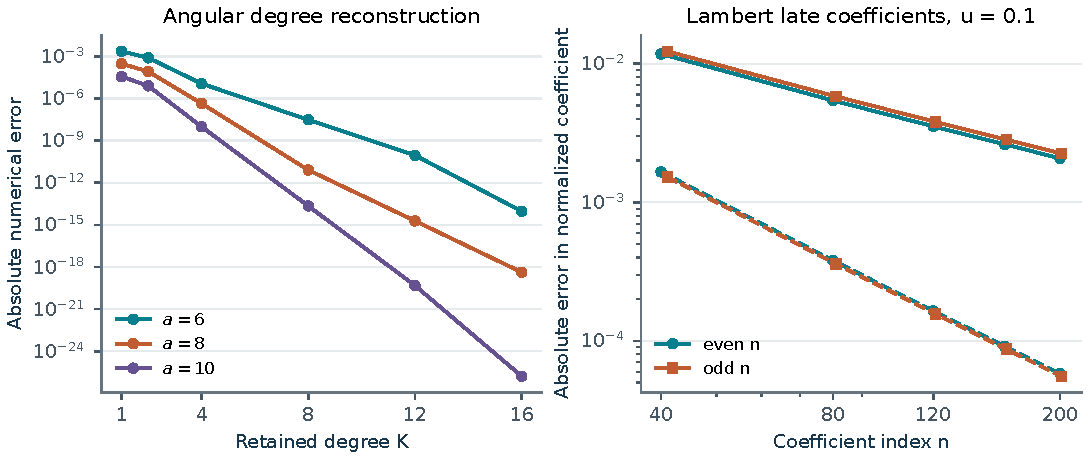
\includegraphics[width=\textwidth]{figures/diagnostics.pdf}
\caption{Numerical consequences of the proofs. Left: angular
degree reconstruction at $b=1$, $\rho=1$. Right: Lambert errors
at $u=0.1$, with even and odd indices separated. Solid curves use
the leading term; dashed curves include the first correction.
Points are diagnostics, not interval certificates.}
\label{fig:diagnostics}
\end{figure}

For the removable endpoint expansions at $y=10^{-3}$, direct
polylogarithm root calculations give polynomial errors approximately
$1.7191\cdot10^{-19}$ for \eqref{ep:eq:q2} and
$1.0461\cdot10^{-29}$ for \eqref{ep:eq:q3}. Four cut-bank tests
compare direct evaluation with an independently formed Jonqui\`ere
expansion. The local threshold is proved using exact sign estimates;
the decimals only check normalization and branch conventions.

\subsection{Recommended changes to the existing material}

No incorrect theorem was found in the particular angular finite-cutoff,
angular divergence, integer cut-modulus, or Lambert coefficient
statements used here. The justified integration changes are:
\begin{enumerate}
\item Mark the angular summation question as answered for $a\ge6$,
retaining the nonlinear-degree and radial-degree data. Preserve the
source's divergence warning.
\item Add the finite approximation as progress on moving truncation,
while keeping sharp optimality open.
\item Replace the two named Lambert conjectures with
Theorem~\ref{lm:thm:sharp}; cross-reference the first correction
and Borel decomposition. Extend the exact-radius assertion in this
model to every complex $u\ne0$.
\item Add the minimal direct-inverse ramification classification as
a refinement of the existing noninteger charts.
\item Record the failure of the all-real cut-modulus extension for
$1<s<3/2$ and the sharp local threshold. Retain the integer-order
theorem; leave both the global noninteger cut-modulus range and the
broader endpoint-circle question open.
\end{enumerate}
These are changes of mathematical status and scope. Correct historical
reports need not be rewritten, and an open question should not be
described as an erroneous theorem.

\section{Further research questions}
\label{sec:future}

\subsection{Angular summation and finite approximation}

\paragraph{1. Find the least uniform outer-order threshold.}
Determine the least $a_*$ for convergence of the scalar coupling
Taylor series at $\tau=1$, uniformly in $b>0$ and $0<\rho\le1$.
The explicit $a\ge6$ uses a simple disk and rational constants.
A sharper norm may still miss the true obstruction: a complex
coupling singularity satisfying $v=\tau f(v)$ and
$1=\tau f'(v)$, or a collision with the polylogarithm cut.

\paragraph{2. Prove a sharp optimal truncation law.}
Theorem~\ref{ang:thm:gaussian} attains every
$\lambda<\log(3/2)$ in its Gaussian exponent for one double
cutoff. Determine the sharp error for the original single
exponential-base cutoff and compare the two schemes. A lower bound
must account for the prime-frequency divergence mechanism.

\paragraph{3. Compare natural summation prescriptions.}
Compare analytic continuation in the scalar coupling, radial Abel
degree summation, and limits of exact finite-Fourier roots.
Agreement must be proved in a common domain. A summation method
depending only on coefficients already grouped by exponential base
is a separate problem because the present construction retains
additional multiset data.

\paragraph{4. Reduce the fixed period algebra.}
Use the repository's cyclotomic and depth-reduction identities to
reduce the generating set in \eqref{ang:eq:algebra}. This asks for
proved reductions, not numerical independence. Compact generator
lists could simplify many consecutive coupling coefficients.

\paragraph{5. Extend to other colors and depths.}
The local construction needs a simple dominant zero and a controlled
complex tail. Identifying it with the intended global geometric zero
requires a separate global theorem. Keep those tasks distinct when
studying other root-of-unity colors or higher-depth harmonic sums.

\subsection{Factorial reversion and Borel geometry}

\paragraph{6. Determine the full inverse Borel continuation.}
Does the inverse Borel germ continue along every path avoiding an
explicit additive action set? The log--dilog decomposition only
describes the initial disk and its boundary regularity. A continuation
theorem should separate inherited arithmetic singularities from those
created by nonlinear convolution.

\paragraph{7. Derive all relative late terms.}
The leading amplitudes detect $r_1$; the next term also detects
$r_2$ and the quadratic core. Prove exactly which finite forward
and core data determine each coefficient of $n^{-j}$ and give a
recursive formula. Borinsky's framework~\cite{Borinsky} is a
natural starting point, with the two-action parity kept explicit.
Successive terms should lead to higher polylogarithms in a refined
initial-disk decomposition.

\paragraph{8. Resolve physical moving-parameter limits.}
The physical inverse has $u=1/X$ and $q=e^{\gamma-X}$.
A useful optimal-truncation analysis must choose $n$ jointly with
$X$. Derive the transition between the action amplitudes as $u\to0$
and quantify the smallest remainder on that physical curve.

\paragraph{9. Study cancellation of a parity amplitude.}
At imaginary couplings an even or odd leading amplitude can vanish.
Classify the first nonzero late term on each such locus. The
first correction is a starting point; the cancellation of one
parity amplitude does not remove either individual logarithmic action.

\subsection{Global inverse geometry}

\paragraph{10. Determine the global cut-modulus range.}
The threshold $s=3/2$ is exact locally. For which noninteger
real $s\ge3/2$ does the strict inequality persist for every
$u>0$? Control the entire cut and distinguish the chosen
principal-sheet image boundary from intrinsic inverse singularities.

\paragraph{11. Locate the nearest singularities at exceptional orders.}
At $s=1+1/q$, $\zeta(s)$ is regular for the continued inverse,
with a critical point of order $q$. What controls the Taylor
radius of the original germ at $w=0$? Candidates include critical
values on other sheets and finite asymptotic values. The local
removability theorem does not choose among them.

\paragraph{12. Compare direct and feedback ramification.}
Seek a local classification for $\Psi(v)=\Li_s(\Phi(v))$
with prescribed vanishing orders of $\Psi$ and $\Phi-1$.
Quadratic feedback can change the direct degree $\min(p,q)$ and
create folds. Resonant logarithms must be treated separately from
rational powers; deleting them can produce a false finite-cover claim.

\paragraph{13. Formalize the reusable finite algebra.}
The finite factorial convolution inequalities, coefficient extraction,
parity formulas, and rational norm certificates are suitable first
formalization targets. Full analytic formalization also needs the
polylogarithm continuation and kernel machinery, and the relevant
complex-analytic theorems. This package makes no claim that those
prerequisites or the present proofs have already been formalized.

\begin{thebibliography}{99}

\bibitem{Gessel}
I.~M.~Gessel, \emph{Lagrange inversion},
Journal of Combinatorial Theory, Series A \textbf{144} (2016), 212--249.
\href{https://doi.org/10.1016/j.jcta.2016.06.018}{doi:10.1016/j.jcta.2016.06.018};
\href{https://arxiv.org/abs/1609.05988}{arXiv:1609.05988}.

\bibitem{Borinsky}
M.~Borinsky, \emph{Generating asymptotics for factorially divergent
sequences}, Electronic Journal of Combinatorics \textbf{25}(4)
(2018), Paper~4.1.
\href{https://arxiv.org/abs/1603.01236}{arXiv:1603.01236};
\href{https://www.combinatorics.org/ojs/index.php/eljc/article/download/v25i4p1/pdf/}{published open-access paper}.

\bibitem{DK}
D.~Dorigoni and A.~Kleinschmidt,
\emph{Resurgent expansion of Lambert series and iterated Eisenstein
integrals}, Communications in Number Theory and Physics \textbf{15}
(2021), 1--57.
\href{https://arxiv.org/abs/2001.11035}{arXiv:2001.11035}.

\bibitem{DLMF}
NIST, \emph{Digital Library of Mathematical Functions},
\S25.12, especially equations 25.12.11--25.12.12.
\url{https://dlmf.nist.gov/25.12}. Accessed 12 October 2026.

\bibitem{RepoAngular}
\repo\ research corpus, \emph{Angular-zero continuation},
\path{Analysis/Polylogarithms/docs/reports/angular-zero-continuation/article.tex}.
Theorem \texttt{thm:allorders}, equation
\texttt{eq:lagrange-coefficient}, and remark
\texttt{rem:not-convergent}.
\href{https://github.com/VladimirReshetnikov/ProveIt/blob/8f5afd4d7565df808359f6a0c22f87f79a119bb9/Analysis/Polylogarithms/docs/reports/angular-zero-continuation/article.tex}{Pinned source}.

\bibitem{RepoFormal}
\repo\ research corpus, \emph{Formal reductions continuation},
\path{Analysis/Polylogarithms/docs/reports/formal-reductions-continuation/article/sections/}.
Files \texttt{angular\_divergence.tex} and \texttt{research.tex};
theorem \texttt{angular:thm:divergence} and research questions 13--14.
\href{https://github.com/VladimirReshetnikov/ProveIt/tree/8f5afd4d7565df808359f6a0c22f87f79a119bb9/Analysis/Polylogarithms/docs/reports/formal-reductions-continuation/article/sections}{Pinned source directory}.

\bibitem{RepoThreshold}
\repo\ research corpus, \emph{Real-order threshold},
\path{Analysis/Polylogarithms/docs/reports/real-order-threshold/article/real_order_threshold.tex}.
Theorems \texttt{thm:double} and \texttt{thm:angular},
corollary \texttt{cor:gaussian}.
\href{https://github.com/VladimirReshetnikov/ProveIt/blob/8f5afd4d7565df808359f6a0c22f87f79a119bb9/Analysis/Polylogarithms/docs/reports/real-order-threshold/article/real_order_threshold.tex}{Pinned source}.

\bibitem{RepoLambert}
\repo\ incoming research report, \emph{Resonant Lambert inverse
transseries}, archive
\path{Resonant_Lambert_Inverse_Transseries_2026-10-12.zip},
member \path{Resonant_Lambert_Inverse_Transseries/article.tex}.
Equations \texttt{eq:C-formula}, \texttt{eq:conj-even},
\texttt{eq:conj-odd}; theorem \texttt{thm:inverse-gevrey}.
\href{https://github.com/VladimirReshetnikov/ProveIt/blob/8f5afd4d7565df808359f6a0c22f87f79a119bb9/docs/incoming/Resonant_Lambert_Inverse_Transseries_2026-10-12.zip}{Pinned incoming archive}.

\bibitem{RepoInverse}
\repo\ research corpus, \emph{Polylogarithm resonance and inverse
transseries},
\path{Analysis/Transseries/docs/series-and-transseries/Polylogarithm_Resonance_And_Inverse_Transseries/polylogarithm_resonance_and_inverse_transseries.tex}.
Proposition \texttt{prop:noninteger}, lemma \texttt{lem:cutgap},
and further research question~9.
\href{https://github.com/VladimirReshetnikov/ProveIt/blob/8f5afd4d7565df808359f6a0c22f87f79a119bb9/Analysis/Transseries/docs/series-and-transseries/Polylogarithm_Resonance_And_Inverse_Transseries/polylogarithm_resonance_and_inverse_transseries.tex}{Pinned source}.

\bibitem{RepoQuadratic}
\repo\ incoming research report,
\emph{Quadratic polylogarithm boundaries}, archive
\path{ProveIt_Quadratic_Polylog_Boundaries_2026-10-12.zip},
member \path{ProveIt_Quadratic_Polylog_Boundaries_2026-10-12/article.tex}.
\href{https://github.com/VladimirReshetnikov/ProveIt/blob/8f5afd4d7565df808359f6a0c22f87f79a119bb9/docs/incoming/ProveIt_Quadratic_Polylog_Boundaries_2026-10-12.zip}{Pinned incoming archive}.

\bibitem{RepoJets}
\repo\ incoming research report,
\emph{Lambert polylogarithm order jets}, archive
\path{ProveIt_Lambert_Polylog_Order_Jets_2026-10-12.zip},
member \path{lambert_polylog_order_jets/main.tex}.
Inspected for overlap in the present source audit.
\href{https://github.com/VladimirReshetnikov/ProveIt/blob/8f5afd4d7565df808359f6a0c22f87f79a119bb9/docs/incoming/ProveIt_Lambert_Polylog_Order_Jets_2026-10-12.zip}{Pinned incoming archive}.
\end{thebibliography}

\end{document}
